%!TEX root = ../out/08-MC-SL.tex

\usepackage{alltt}

\begin{document}

\mytitle{Measure \& Conquer}{Measure \& Conquer}

\section{Introduction}

\begin{frame}{Recall: Maximal Independent Sets}
  %\pause
  \begin{itemize}
   \item A vertex set $S\subseteq V$ of a graph $G=(V,E)$ is an \alert{independent set} in $G$ if there is no edge $uv\in E$ with $u,v\in S$.
   \item An independent set is \alert{maximal} if it is not a subset of any other independent set.
   \item Examples:

  \begin{center}
   \begin{tikzpicture}[scale=0.7]
      \node[selected] (a) at (1.5,3  ) {};
      \node[vertex]   (b) at (3  ,3  ) {};
      \node[vertex]   (c) at (0  ,1.5) {};
      \node[vertex]   (d) at (1.5,1.5) {};
      \node[vertex]   (e) at (3  ,1.5) {};
      \node[vertex]   (f) at (1.5,0  ) {};
      \node[selected] (g) at (3  ,0  ) {};
      \node[vertex]   (h) at (4.5,0  ) {};
    \draw[line width=2pt]     (a) -- (b) -- (e) -- (h) -- (g) -- (f) -- (d) -- (g) -- (e) -- (a) -- (c) -- (d) -- (a);
   \end{tikzpicture}
   \begin{tikzpicture}[scale=0.7]
      \node[vertex]   (a) at (1.5,3  ) {};
      \node[selected] (b) at (3  ,3  ) {};
      \node[selected] (c) at (0  ,1.5) {};
      \node[vertex]   (d) at (1.5,1.5) {};
      \node[vertex]   (e) at (3  ,1.5) {};
      \node[selected] (f) at (1.5,0  ) {};
      \node[vertex]   (g) at (3  ,0  ) {};
      \node[selected] (h) at (4.5,0  ) {};
    \draw[line width=2pt]     (a) -- (b) -- (e) -- (h) -- (g) -- (f) -- (d) -- (g) -- (e) -- (a) -- (c) -- (d) -- (a);
   \end{tikzpicture}
  \end{center}
  \end{itemize}

\end{frame}

\begin{frame}
 \frametitle{Enumeration problem: Enumerate all maximal independent sets}

 \pbDefOpt{\textsc{Enum-MIS}}{graph $G$}{all maximal independent sets of $G$}
 
 \begin{center}
  \begin{tikzpicture}[scale=1]
       \node[vertex,label=above:$a$] (a) at (  0,1.5) {};
       \node[vertex,label=above:$b$] (b) at (1.5,1.5) {};
       \node[vertex,label=below:$c$] (c) at (  0,  0) {};
       \node[vertex,label=below:$d$] (d) at (1.5,  0) {};
       \draw[line width=1.5pt] (c)--(a) -- (b) -- (d) -- (c) -- (b);
  \end{tikzpicture}
 \end{center}
 Maximal independent sets: $\{a,d\}, \{b\}, \{c\}$
 
 \medskip
 \pause\noindent
 \textbf{Note:} Let $v$ be a vertex of a graph $G$. Every maximal independent set contains a vertex from $N_G[v]$.

\end{frame}


\begin{frame}
 \frametitle{Branching Algorithm for \textsc{Enum-MIS}}

\begin{algorithm}[H]
\DontPrintSemicolon
\SetArgSty{}
\alert{Algorithm $\text{\algenummis}(G,I)$}\;
\SetKwInOut{Input}{Input}
\SetKwInOut{Output}{Output}
\Input{A graph $G=(V,E)$, an independent set $I$ of $G$.}
\Output{All maximal independent sets of $G$ that are supersets of $I$.}
\BlankLine
   \lnl{algenummis1:0}$G' \leftarrow G - N_G[I]$\;
   \lnl{algenummisl:3}\If(\tcp*[f]{$G'$ has no vertex}){$V(G')=\emptyset$} {
      \lnl{algenummisl:4} \textbf{Output} $I$\;
   }
   \lnl{algenummisl:5}\Else {
      \lnl{algenummisl:6}Select $v \in V(G')$ such that $d_{G'}(v) = \delta(G')$\tcp*[f]{$v$ has min degree in $G'$}\;
      \lnl{algenummisl:7}\textbf{Run} $\text{\algenummis}(G,I\cup \{u\})$ for each $u\in N_{G'}[v]$\;
   }
\end{algorithm}

\end{frame}


\begin{frame}
	\frametitle{Running Time Analysis}
	
	Let $L(n)=2^{\alpha n}$ be an upper bound on the number of leaves in any search tree of \algenummis for an instance with $|V(G')|\le n$.
	
	\medskip
	\noindent
	We minimize $\alpha$ subject to constraints obtained from the branching:
	%
	\begin{align*}
	&&L(n) &\ge (d+1) \cdot L(n - (d+1)) && \text{for each integer $d\ge 0$.}\\
	&\Leftrightarrow& 2^{\alpha n} &\ge d' \cdot 2^{\alpha \cdot (n-d')} && \text{for each integer $d'\ge 1$.}\\
	&\Leftrightarrow& 1 &\ge d' \cdot 2^{\alpha \cdot (-d')} && \text{for each integer $d'\ge 1$.}
	\end{align*}
	%
	\noindent
	For fixed $d'$, the smallest value for $2^\alpha$ satisfying the constraint is $d'^{1/d'}$. The function $f (x)=x^{1/x}$ has its maximum value for $x=e$ and for integer
	$x$ the maximum value of $f (x)$ is when $x = 3$.
	
	Therefore, the minimum value for $2^\alpha$ for which all constraints hold is $3^{1/3}$. We can thus set $L(n)=3^{n/3}$.
	
\end{frame}

\begin{frame}
 \slides{\frametitle{Running Time Analysis II}}
 
 \lecturenotes{\medskip}
 \noindent
 Since the height of the search trees is $\le |V(G')|$, we obtain:
 
 \begin{theorem}
  Algorithm $\text{\algenummis}$ has running time $O^*(3^{n/3}) \subseteq O(1.4423^n)$, where $n=|V|$.
 \end{theorem}
 
 \begin{corollary}
  A graph on $n$ vertices has $O(3^{n/3})$ maximal independent sets.
 \end{corollary}
 
\end{frame}



\begin{frame}
 \frametitle{Running Time Lower Bound}
 
  \begin{center}
   \begin{tikzpicture}
    \foreach \x in {1,3,5,9}
      \draw (\x,0) node[vertex] {} -- (\x+1,0) node[vertex] {} -- (\x+0.5,1) node[vertex] {} -- cycle;
    \draw (7.5,0.5) node {$\cdots$};
   \end{tikzpicture}
  \end{center}
  
  \begin{theorem}
   There is an infinite family of graphs with $\Omega(3^{n/3})$ maximal independent sets.
  \end{theorem}

\end{frame}


\section{Maximum Independent Set}

\begin{frame}
  \slides{\frametitle{\textsc{Maximum Independent Set}}}

 \pbDefOpt{\textsc{Maximum Independent Set}}{graph $G$}{A largest independent set of $G$.}

 \begin{center}
 \begin{tikzpicture}[scale=0.7]
      \node[vertex]  (a) at (1.5,3  ) {};
      \node[selected] (b) at (3  ,3  ) {};
      \node[selected] (c) at (0  ,1.5) {};
      \node[vertex]                 (d) at (1.5,1.5) {};
      \node[vertex]                 (e) at (3  ,1.5) {};
      \node[selected] (f) at (1.5,0  ) {};
      \node[vertex]                 (g) at (3  ,0  ) {};
      \node[selected] (h) at (4.5,0  ) {};
      \draw[line width=1.5pt]     (a) -- (b) -- (e) -- (h) -- (g) -- (f) -- (d) -- (g) -- (e) -- (a) -- (c) -- (d) -- (a);
 \end{tikzpicture}
 \end{center}

\end{frame}


\begin{frame}
 \frametitle{Branching Algorithm for \textsc{Maximum Independent Set}}
 
\begin{algorithm}[H]
\DontPrintSemicolon
\SetArgSty{}
%
\alert{Algorithm $\text{\algmis}(G)$}\;
\SetKwInOut{Input}{Input}
\SetKwInOut{Output}{Output}
\Input{A graph $G=(V,E)$.}
\Output{The size of a \mis of $G$.}
\BlankLine
%
   \lnl{algmisl:1}\If(\tcp*[f]{$G$ has max degree $\le 2$}){$\Delta(G) \le 2$} {
      \lnl{algmisl:2}\Return{the size of a \mis of $G$ in polynomial time}\;
   }
   \lnl{algmisl:3}\ElseIf(\tcp*[f]{$v$ has degree $1$}){$\exists v \in V: d(v) = 1$} {
      \lnl{algmisl:4}\Return{$1+\text{\algmis}(G - N[v]$)}\;
   }
   \lnl{algmisl:5}\ElseIf{$G$ is not connected} {
      \lnl{algmisl:5a}Let $G_1$ be a connected component of $G$\;
      \lnl{algmisl:6}\Return{$\text{\algmis}(G_1) + \text{\algmis}(G - V(G_1))$}\;
   }
   \lnl{algmisl:7}\Else {
      \lnl{algmisl:8}Select $v \in V$ s.t. $d(v) = \Delta(G)$ \tcp*[f]{$v$ has max degree}\;
      \lnl{algmisl:9}\Return{$\max \left( 1+\text{\algmis}(G - N[v]), \text{\algmis}(G - v) \right)$}\;
   }
%\caption{Algorithm $\text{\algmis}(G)$, computing the size of a maximum independent set of any input graph $G$\index{algorithm!mis@\algmis}}
\end{algorithm}

\end{frame}

\begin{frame}
	\frametitle{Correctness}
	
	Line \ref{algmisl:4}:
	\begin{lemma}
		If $v\in V$ has degree 1, then $G$ has a maximum independent set $I$ with $v\in I$.
	\end{lemma}
	\begin{proof}
		Let $J$ be a maximum independent set of $G$.\\
		If $v\in J$ we are done because we can take $I=J$.\\
		If $v\notin J$, then $u\in J$, where $u$ is the neighbor of $v$, otherwise $J$ would not be maximum.\\
		Set $I=(J\setminus \{u\})\cup \{v\}$. We have that $I$ is an independent set, and, since $|I|=|J|$, $I$ is a maximum independent set containing $v$.
	\end{proof}
	
\end{frame}

\subsection{Simple Analysis}

\begin{frame}[allowframebreaks]
 \slides{\frametitle{Simple Analysis}}

\begin{lemma}[Simple Analysis Lemma] \label{lem:simpleanalysis}
Let
\begin{itemize}
 \item $A$ be a branching algorithm
 \item $\alpha > 0, \; c \ge 0$ be constants
\end{itemize}
such that
on input $I$, $A$ calls itself recursively on instances $I_1,\ldots,I_k$, but, besides the recursive calls, uses time $\cO(|I|^c)$, such that
\begin{align}
(\forall i: 1 \le i \le k) \quad |I_i| & \leq |I|-1 \text{, and}  \label{eq:sasize}
  \\
2^{\alpha \cdot |I_1|} + \cdots + 2^{\alpha \cdot |I_k|} & \leq 2^{\alpha \cdot |I|} . \label{eq:sagain}
\end{align}
Then $A$ solves any instance $I$
in time $\cO(|I|^{c+1}) \cdot 2^{\alpha \cdot |I|}$.
\end{lemma}

\framebreak

\begin{proof}
By induction on $|I|$.\\
W.l.o.g., suppose the
hypotheses' $\cO$ statements hide a constant factor $d\ge 0$, and for the base case assume that
the algorithm returns the solution to an empty instance in time $d \le d\cdot |I|^{c+1} 2^{\alpha \cdot |I|}$.

Suppose the lemma holds for all instances of size at most $|I|-1\ge 0$, then the running time of algorithm $A$ on instance $I$ is
{\allowdisplaybreaks
\begin{align*}
T_A(I) & \le d\cdot |I|^c + \sum_{i=1}^k T_A(I_i) 
  &\text{\quad (by definition)}
\\ &\le d\cdot |I|^c + \sum d\cdot |I_i|^{c+1} 2^{\alpha \cdot |I_i|} 
  &\text{\quad (by the inductive hypothesis)}
% \\ &\leq |F|^k \sum 2^{\mu(F_i)} \text{ (as long as every $|F_i| \leq |F|-1$)}
\\ &\le d\cdot |I|^c + d\cdot (|I|-1)^{c+1} \sum 2^{\alpha \cdot |I_i|}
  &\text{\quad (by \eqref{eq:sasize})}
\\ &\le d\cdot |I|^c + d\cdot (|I|-1)^{c+1} 2^{\alpha \cdot |I|} 
  &\text{\quad (by \eqref{eq:sagain})}
% \\ &\leq |F|^k 2^{\mu(F)} \text{ (by hypothesis \eqref{mu})}.
\\ &\le d\cdot |I|^{c+1} 2^{\alpha \cdot |I|} .
%  \text{ (following from $k \geq 1$).}
\end{align*}}
The final inequality uses that $\alpha \cdot |I| > 0$ and holds for any $c \geq 0$.
\end{proof}

\end{frame}

\begin{frame}
 \frametitle{Simple Analysis for \algmis}

 \begin{itemize}
  \item At each node of the search tree: $\cO(n^2)$ time
  \item $G$ disconnected: let $s:= |V(G_1)|$\\
  (1) If $\alpha\cdot s<1$, then $s<1/\alpha$, and the algorithm solves $G_1$ in constant time (provided that $\alpha>0$). We can view this rule as a simplification rule, removing $G_1$ and making one recursive call on $G-V(G_1)$.\\
  (2) If $\alpha \cdot (n-s)<1$: similar as (1).\\
  (3) Otherwise,
\begin{align}
 (\forall s: 1/\alpha \le s \le n-1/\alpha) \quad 2^{\alpha \cdot s} + 2^{\alpha \cdot (n-s)} \leq 2^{\alpha \cdot n}.
\end{align}
  always satisfied since $2^x+2^y \le 2^{x+y}$ if $x,y\ge 1$.

  \item Branch on vertex of degree $d \ge 3$
\begin{align}
 (\forall d: 3 \le d \le n-1) \quad 2^{\alpha \cdot (n-1)} + 2^{\alpha \cdot (n-1-d)} &\leq 2^{\alpha n}.
\intertext{%
Dividing all these terms by $2^{\alpha n}$, the constraints become}
 2^{-\alpha} + 2^{\alpha \cdot (-1-d)} &\leq 1.
 \label{eq:mis1constraints}
\end{align}
\end{itemize}
\end{frame}


\begin{frame}
 \frametitle{Compute optimum $\alpha$}
 
 \noindent
 The minimum $\alpha$ satisfying the
constraints is obtained by 
solving a convex mathematical program minimizing $\alpha$ subject
to the constraints (the constraint for $d=3$ is sufficient as
all other constraints are weaker).

\pause
\medskip\noindent
Alternatively, set $x:=2^{\alpha}$, compute the unique
positive real root of each of the \alert{characteristic polynomials}
\begin{align*}
 c_d(x) := x^{-1} + x^{-1-d} - 1,
\end{align*}
and take the maximum of these roots \cite{Kullmann99}.
%
\begin{align*}
\begin{array}{|c|c|c|}
\hline
d & \quad x & \quad \alpha\\
\hline
3 & \quad 1.3803 & \quad 0.4650 \\
4 & \quad 1.3248 & \quad 0.4057 \\
5 & \quad 1.2852 & \quad 0.3620 \\
6 & \quad 1.2555 & \quad 0.3282 \\
7 & \quad 1.2321 & \quad 0.3011 \\
\hline
\end{array}
\end{align*}
\end{frame}


\begin{frame}
 \frametitle{Simple Analysis: Result}

 \begin{itemize}
 \item use the Simple Analysis Lemma with $c=2$ and $\alpha = 0.464959$
 \item running time of Algorithm~\algmis upper bounded by
$\cO(n^3) \cdot 2^{0.464959 \cdot n} = \cO(2^{0.4650 \cdot n})$ or $\cO(1.3803^n)$
 \end{itemize}
 
\end{frame}


\begin{frame}
 \frametitle{Lower bound}

\begin{center}
 \begin{tikzpicture}[scale=1]

   \draw (0,0) node[vertex,label=below:$v_1$] (v1) {};
   \draw (1,0) node[vertex,label=below:$v_2$] (v2) {};
   \draw (2,0) node[vertex,label=below:$v_3$] (v3) {};
   \draw (3,0) node[vertex,label=below:$v_4$] (v4) {};
   \draw (4,0) node[vertex,label=below:$v_5$] (v5) {};
   \draw (5,0) node[vertex,label=below:$v_6$] (v6) {};
   \draw (7,0) node[vertex,label=below:$v_{n-1}$] (vs) {};
   \draw (8,0) node[vertex,label=below:$v_n$] (vn) {};
   
   \draw (v1)--(v2)--(v3)--(v4)--(v5)--(v6) (vs)--(vn);
   \draw (v1) .. controls +(0,1) and +(0,1) .. (v3);
   \draw (v2) .. controls +(0,1) and +(0,1) .. (v4);
   \draw (v3) .. controls +(0,1) and +(0,1) .. (v5);
   \draw (v4) .. controls +(0,1) and +(0,1) .. (v6);
   \begin{scope}
    \clip (4,0) rectangle (5,1);
    \draw (v5) .. controls +(0,1) and +(0,1) .. (6,0);
   \end{scope}
   \begin{scope}
    \clip (7,0) rectangle (8,1);
    \draw (6,0) .. controls +(0,1) and +(0,1) .. (vn);
   \end{scope}

   \filldraw (5.8,0) circle (0.2mm);
   \filldraw (6.0,0) circle (0.2mm);
   \filldraw (6.2,0) circle (0.2mm);
  
 \end{tikzpicture}
\end{center}

 \begin{align*}
  T(n) = T(n-5) + T(n-3)
 \end{align*}

 \begin{itemize}
  \item for this graph, $P_n^2$, the worst case running time is $1.1938\ldots^n \cdot \mathsf{poly}(n)$
  \item Run time of algo \algmis is $\Omega(1.1938^n)$
 \end{itemize}

\end{frame}

\begin{frame}
 \frametitle{Worst-case running time --- a mystery}
 
 \begin{block}{\slides{Mystery}}
  What is the worst-case running time of Algorithm \algmis?
 \end{block}
 
 \begin{itemize}
  \item lower bound $\Omega(1.1938^n)$
  \item upper bound $\cO(1.3803^n)$
 \end{itemize}

\end{frame}


\subsection{Search Trees and Branching Numbers}

\begin{frame}
 \frametitle{Search Trees}

 \lecturenotes{\medskip}
 \noindent
 Denote $\mu(I) := \alpha \cdot |I|$.
 
 \begin{center}
 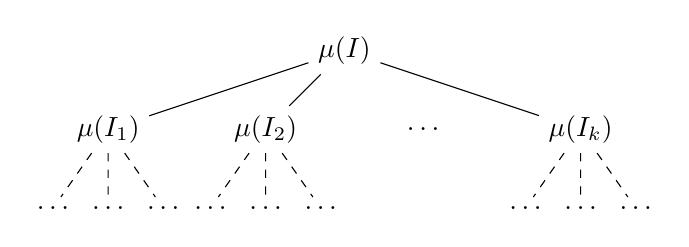
\begin{tikzpicture}[scale=1,level distance=10mm]
  \tikzstyle{level 1}=[sibling distance=20mm]
  \tikzstyle{level 2}=[sibling distance=7mm]
  \node {$\mu(I)$}
   child {node {$\mu(I_1)$}
    child[dashed] {node {$\dots$}}
    child[dashed] {node {$\dots$}}
    child[dashed] {node {$\dots$}}
   }
   child {node {$\mu(I_2)$}
    child[dashed] {node {$\dots$}}
    child[dashed] {node {$\dots$}}
    child[dashed] {node {$\dots$}}
   }
   child {node {$\dots$} edge from parent[draw=none]}
   child {node {$\mu(I_k)$}
    child[dashed] {node {$\dots$}}
    child[dashed] {node {$\dots$}}
    child[dashed] {node {$\dots$}}
   }
  ;
 \end{tikzpicture}
 \end{center}

 \medskip\pause\noindent
 Example: execution of \algmis on a $P_n^2$

 \begin{center}
 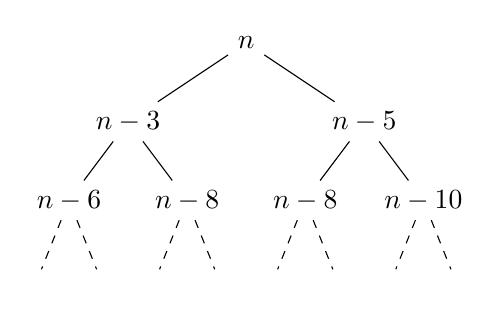
\begin{tikzpicture}[scale=1,level distance=10mm]
  \tikzstyle{level 1}=[sibling distance=30mm]
  \tikzstyle{level 2}=[sibling distance=15mm]
  \tikzstyle{level 3}=[sibling distance=8mm]
  \node {$n$}
   child {node {$n-3$}
    child {node {$n-6$}
     child[dashed] {node {}}
     child[dashed] {node {}}
    }
    child {node {$n-8$}
     child[dashed] {node {}}
     child[dashed] {node {}}
    }
   }
   child {node {$n-5$}
    child {node {$n-8$}
     child[dashed] {node {}}
     child[dashed] {node {}}
    }
    child {node {$n-10$}
     child[dashed] {node {}}
     child[dashed] {node {}}
    }
   }
  ;
 \end{tikzpicture}
 \end{center}
\end{frame}


\begin{frame}
 \frametitle{Branching number: Definition}
 
 \lecturenotes{\medskip}
 \noindent
 Consider a constraint
\begin{align*}
 2^{\mu(I)-a_1} + \cdots + 2^{\mu(I)-a_k} & \leq 2^{\mu(I)}.
\end{align*}
Its \alert{branching number} is
\begin{align*}
 2^{-a_1} + \cdots + 2^{-a_k},
\end{align*}
and is denoted by
\begin{align*}
 \left(a_1, \ldots, a_k\right).
\end{align*}
Clearly, any constraint with branching number at most $1$ is satisfied.
\end{frame}

\begin{frame}
 \frametitle{Branching numbers: Properties}
 
\begin{description}
 \item[Dominance] For any $a_i, b_i$ such that $a_i \ge b_i$ for all $i, \; 1 \le i \le k$,
  \begin{align*}
   \left(a_1, \ldots, a_k\right) \le \left(b_1, \ldots, b_k\right),
  \end{align*}
  as $2^{-a_1}+\cdots+2^{-a_k} \le 2^{-b_1}+\cdots+2^{-b_k}$. \newline
  %We say in this case that the branching number $\left(a_1, \ldots, a_k\right)$ is \emph{dominated} by the branching number $\left(b_1, \ldots, b_k\right)$.
  In particular, for any $a,b > 0$,
  \begin{align*}
   \text{either } \quad \left(a,a\right) \le \left(a,b\right) \quad \text{ or } \quad \left(b,b\right) \le \left(a,b\right).
  \end{align*}
 \item[Balance] If $0 < a \le b$, then for any $\varepsilon$ such that $0 \le \varepsilon \le a$,
  \begin{align*}
   \left( a,b \right) \le \left( a - \varepsilon, b + \varepsilon \right)
  \end{align*}
  by convexity of $2^x$.
  % We say in this case that $\left( a,b \right)$ is more \emph{balanced} than $\left( a - \varepsilon, b + \varepsilon \right)$.
\end{description}
\end{frame}


\subsection{Measure \& Conquer Analysis}

\begin{frame}
 \slides{\frametitle{Measure \& Conquer analysis}}
 
 \begin{itemize}
  \item Goal
   \begin{itemize}
    \item capture more structural changes when branching into subinstances
   \end{itemize}
  \item How?
   \begin{itemize}
    \item via a potential-function method called \alert{Measure \& Conquer}
          \cite{FominGK09}
   \end{itemize}
  \item Example: Algorithm \algmis
  \begin{itemize}
   \item advantage when degrees of vertices decrease
  \end{itemize}
 \end{itemize}
 
\end{frame}

\begin{frame}
	\frametitle{Measure}
	
  Instead of using the number of vertices, $n$, to track the progress of \algmis, let us use a measure $\mu$ of $G$.

  \begin{definition}
    A \alert{measure} $\mu$ for a problem $P$ is a function from the set of all instances for $P$ to the set of non negative reals.
  \end{definition}

  Let us use the following measure for the analysis of \algmis on graphs of maximum degree at most 5:
   \begin{align*}
    \mu(G) = \sum_{i=0}^5 \omega_i n_i,
   \end{align*}
   where $n_i:=|\{v\in V: d(v)=i\}|$.

\end{frame}


\begin{frame}
	\frametitle{Measure \& Conquer Analysis}
	
	\begin{lemma}[Measure \& Conquer Lemma]\label{lem:measure-analysis}
		Let
		\begin{itemize}
			\item $A$ be a branching algorithm
			\item $c \ge 0$ be a constant, and
			\item $\mu(\cdot), \eta(\cdot)$ be two measures
			for the instances of $A$,
		\end{itemize}
		such that
		on input $I$, $A$ calls itself recursively on instances $I_1,\ldots,I_k$, but, besides the recursive calls, uses time $\cO(\eta(I)^c)$, such that
		\begin{align}
		(\forall i) \quad \eta(I_i) & \leq \eta(I)-1 \text{, and}  \label{eq:masize}
		\\
		2^{\mu(I_1)} + \ldots + 2^{\mu(I_k)} & \leq 2^{\mu(I)} . \label{eq:magain}
		\end{align}
		Then $A$ solves any instance $I$
		in time $\cO(\eta(I)^{c+1}) \cdot 2^{\mu(I)}$.
	\end{lemma}
	
\end{frame}


\begin{frame}
 \frametitle{Analysis of mis for degree at most 5}
 
 For $\mu(G) = \sum_{i= 0}^5 \omega_i n_i$ to be a valid measure, we constrain that
 \begin{align*}
   w_d &\ge  0 && \text{for each }d\in\{0,\dots,5\}
 \end{align*}

 \medskip
 We also constrain that reducing the degree of a vertex does not increase the measure (useful for analysis of the degree-1 simplification rule and the branching rule):
 \begin{align*}
  	-\omega_d+\omega_{d-1} &\le  0 && \text{for each }d\in\{1,\dots,5\}
 \end{align*}

 \medskip
 \pause
 Lines \ref{algmisl:1}--\ref{algmisl:2} is a halting rule and we merely need that it takes polynomial time so that we can apply Lemma \ref{lem:measure-analysis}.
 \slides{\begin{algorithm}[H]
	\DontPrintSemicolon
	\SetArgSty{}
	\If(\tcp*[f]{$G$ has max degree $\le 2$}){$\Delta(G) \le 2$} {
		\Return{the size of a \mis of $G$ in polynomial time}\;
	}
\end{algorithm}}


\end{frame}


\begin{frame}
	\slides{\frametitle{Analysis of mis for degree at most 5 (II)}}

 Lines \ref{algmisl:3}--\ref{algmisl:4} of \algmis need to satisfy \eqref{eq:magain}.
 \slides{\begin{algorithm}[H]
 	\DontPrintSemicolon
 	\SetArgSty{}
 	\ElseIf(\tcp*[f]{$v$ has degree $1$}){$\exists v \in V: d(v) = 1$} {
	 	\Return{$1+\text{\algmis}(G - N[v]$)}\;
 	}
 \end{algorithm}}
 
 The simplification rule removes $v$ and its neighbor $u$.\\
 We get a constraint for each possible degree of $u$:\\
 \begin{align*}
	 &&2^{\mu(G)-\omega_1-\omega_d} &\le 2^{\mu(G)} && \text{for each }d\in \{1,\dots,5\}\\
	 &\Leftrightarrow& 2^{-\omega_1-\omega_d} &\le 2^{0} && \text{for each }d\in \{1,\dots,5\}\\
	 &\Leftrightarrow& -\omega_1-\omega_d &\le 0 && \text{for each }d\in \{1,\dots,5\}\\
 \end{align*}
 These constraints are always satisfied since $\omega_d\ge 0$ for each $d\in\{0,\dots,5\}$.\\
 \textbf{Note:} the degrees of $u$'s other neighbors (if any) decrease, but this degree change does not increase the measure.

\end{frame}


\begin{frame}
	\slides{\frametitle{Analysis of mis for degree at most 5 (III)}}
	
 For lines \ref{algmisl:5}--\ref{algmisl:6} of \algmis we consider two cases.
 \slides{\begin{algorithm}[H]
 	\DontPrintSemicolon
 	\SetArgSty{}
 	\ElseIf{$G$ is not connected} {
	 	Let $G_1$ be a connected component of $G$\;
		\Return{$\text{\algmis}(G_1) + \text{\algmis}(G - V(G_1))$}\;
 	}
 \end{algorithm}}
 
 If $\mu(G_1) < 1$ (or $\mu(G-V(G_1)) < 1$, which is handled similarly), then
 we view this rule as a simplification rule, which takes polynomial time to compute $\text{\algmis}(G_1)$,
 and then makes a recursive call $\text{\algmis}(G - V(G_1))$. To ensure that instances
 with measure $< 1$ can be solved in polynomial time, we constrain that
 \begin{align*}
	w_d &>  0 && \text{for each }d\in\{3,4,5\}
 \end{align*}
 and this will be implied by other constraints.
 
 Otherwise, $\mu(G_1)\ge 1$ and $\mu(G-V(G_1))\ge 1$, and we need to satisfy \eqref{eq:magain}.\\
 Since $\mu(G)=\mu(G_1)+\mu(G-V(G_1))$, the constraints
 \begin{align*}
 2^{\mu(G_1)}+2^{\mu(G-V(G_1))} &\le 2^{\mu(G)}
 \end{align*}
 are always satisfied since the slope of the function $2^x$ is at least $1$ when $x\ge 1$.\\
 (I.e., we get no new constraints on $\omega_1, \dots,\omega_5$.)
 
\end{frame}


\begin{frame}
	\slides{\frametitle{Analysis of mis for degree at most 5 (IV)}}

Lines \ref{algmisl:7}--\ref{algmisl:9} of \algmis need to satisfy \eqref{eq:magain}.
\slides{\begin{algorithm}[H]
	\DontPrintSemicolon
	\SetArgSty{}
	\Else {
		Select $v \in V$ s.t. $d(v) = \Delta(G)$ \tcp*[f]{$v$ has max degree}\;
		\Return{$\max \left( 1+\text{\algmis}(G - N[v]), \text{\algmis}(G - v) \right)$}\;
	}
\end{algorithm}}
 We know that in $G - N[v]$, some vertex of $N^2[v]$ has its degree decreased (unless $G$ has at most 6 vertices, which can be solved in constant time).
 Define
 \begin{align*}
 (\forall d: 2 \le d \le 5) \quad h_d &:= \min_{2 \le i \le d} \left\{ w_i-w_{i-1} \right\}
 \end{align*}
 We obtain the following constraints:
\begin{align*}
 && 2^{\mu(G) - w_d - \sum_{i=2}^d p_i \cdot (w_i-w_{i-1})} +
 2^{\mu(G) - w_d - \sum_{i=2}^d p_i \cdot w_i - h_d} &\le 2^{\mu(G)}\\
 &\Leftrightarrow& 2^{- w_d - \sum_{i=2}^d p_i \cdot (w_i-w_{i-1})} +
 2^{- w_d - \sum_{i=2}^d p_i \cdot w_i - h_d} &\le 1
\end{align*}
for all $d, 3 \le d \le 5$ (degree of $v$), and all $p_i, 2 \le i \le d,$ such that $\sum_{i=2}^d p_i = d$ (number of neighbors of degree $i$).
\end{frame}

\begin{frame}
 \frametitle{Applying the lemma}

Our constraints
\begin{align*}
 w_d &\ge 0\\
 -\omega_d+\omega_{d-1} &\le 0\\
 2^{- w_d - \sum_{i=2}^d p_i \cdot (w_i-w_{i-1})} +
 2^{- w_d - \sum_{i=2}^d p_i \cdot w_i - h_d} &\le 1
\end{align*}
are satisfied by the following values:
\pause
\[
 \begin{array}{ c c c }
  \hline
  i & w_i & h_i\\
  \hline
  1 & 0 & 0\\
  2 & 0.25 & 0.25\\
  3 & 0.35 & 0.10\\
  4 & 0.38 & 0.03\\
  5 & 0.40 & 0.02\\
  \hline
 \end{array}
\]

These values for $w_i$ satisfy all the constraints and $\mu(G) \le 2n/5$ for any graph of max degree $\le 5$.\\
Taking $c=2$ and $\eta(G)=n$, the Measure \& Conquer Lemma shows that \algmis
has run time $\cO(n^3) 2^{2n/5} = \cO(1.3196^n)$ on graphs of max degree
$\le 5$.

\end{frame}

\subsection{Optimizing the measure}

\begin{frame}
 \frametitle{Compute optimal weights}
 
 \begin{itemize}
  \item By convex programming \cite{GaspersS12}
 \end{itemize}
 
 \noindent
 All constraints are already convex, except conditions for $h_d$
 \begin{align*}
 (\forall d: 2 \le d \le 5) \quad h_d &:= \min_{2 \le i \le d} \left\{ w_i-w_{i-1} \right\}\\
 &\downdownarrows\\
 (\forall i,d: 2 \le i \le d \le 5) \quad h_d &\le w_i-w_{i-1}.
 \end{align*}
 Use existing convex programming solvers to find optimum weights.
\end{frame}

\begin{frame}[fragile]
 \frametitle{Convex program in AMPL}
{\scriptsize
 \begin{verbatim}
param maxd integer = 5;
set DEGREES := 0..maxd;
var W {DEGREES} >= 0;  # weight for vertices according to their degrees
var g {DEGREES} >= 0;  # weight for degree reductions from deg i
var h {DEGREES} >= 0;  # weight for degree reductions from deg <= i
var Wmax;              # maximum weight of W[d]

minimize Obj: Wmax;    # minimize the maximum weight

subject to MaxWeight {d in DEGREES}:
  Wmax >= W[d];
subject to gNotation {d in DEGREES : 2 <= d}:
  g[d] <= W[d]-W[d-1];
subject to hNotation {d in DEGREES, i in DEGREES : 2 <= i <= d}:
  h[d] <= W[i]-W[i-1];
subject to Deg3 {p2 in 0..3, p3 in 0..3 : p2+p3=3}:
  2^(-W[3] -p2*g[2] -p3*g[3]) + 2^(-W[3] -p2*W[2] -p3*W[3] -h[3]) <=1;
subject to Deg4 {p2 in 0..4, p3 in 0..4, p4 in 0..4 : p2+p3+p4=4}:
  2^(-W[4] - p2*g[2] - p3*g[3] - p4*g[4])
+ 2^(-W[4] - p2*W[2] - p3*W[3] - p4*W[4] - h[4]) <=1;
subject to Deg5 {p2 in 0..5, p3 in 0..5, p4 in 0..5, p5 in 0..5 :
                 p2+p3+p4+p5=5}:
  2^(-W[5] - p2*g[2] - p3*g[3] - p4*g[4] - p5*g[5])
+ 2^(-W[5] - p2*W[2] - p3*W[3] - p4*W[4] - p5*W[5] - h[5]) <=1;
\end{verbatim}
}
\end{frame}

%OUTDATED
%\begin{frame}[fragile,allowframebreaks]
%	\frametitle{Convex program in Python}
%{\scriptsize
%\begin{verbatim}
%from numpy import *
%from FuncDesigner import oovar, oovars # pip install funcdesigner
%from openopt import NLP # pip install openopt
%
%W = oovars(6)('W')
%g = [0]+[W[i]-W[i-1] for i in range(1,6)]
%h = oovars(6)('h')
%Wmax = oovar('Wmax')
%
%obj = Wmax
%startPoint = {W:[1 for i in range(6)],
%              h:[0 for i in range(6)],
%              Wmax:1}
%q = NLP(obj, startPoint)
%
%for d in range(6): # positive vars
%  q.constraints.append(W[d] >= 0)
%for d in range(6): # Max Weight
%  q.constraints.append(Wmax >= W[d])
%for d in range(2,6): # h notation
%  for i in range(2,d+1):
%    q.constraints.append(h[d] <= W[i]-W[i-1])
%p = [0 for x in range(6)]
%for p[2] in range(4): # Deg 3
%  p[3] = 3-p[2]
%  q.constraints.append(  2**(-W[3]-sum([p[i]*g[i] for i in range(2,4)]))
%                       + 2**(-W[3]-sum([p[i]*W[i] for i in range(2,4)])-h[3])
%                       <=1)
%for p[2] in range(5): # Deg 4
%  for p[3] in range(5-p[2]):
%    p[4] = 4-sum(p[2:4])
%    q.constraints.append(  2**(-W[4]-sum([p[i]*g[i] for i in range(2,5)]))
%                         + 2**(-W[4]-sum([p[i]*W[i] for i in range(2,5)])-h[4])
%                         <=1)
%for p[2] in range(6): # Deg 5
%  for p[3] in range(6-p[2]):
%    for p[4] in range(6-sum(p[2:4])):
%      p[5] = 5-sum(p[2:5])
%      q.constraints.append(  2**(-W[5]-sum([p[i]*g[i] for i in range(2,6)]))
%                           + 2**(-W[5]-sum([p[i]*W[i] for i in range(2,6)])-h[5])
%                           <=1)
%q.ftol = 1e-10
%q.xtol = 1e-10
%r = q.solve('ralg') # use pyipopt for better performance
%Wmax_opt = r(Wmax)
%print(r.xf)
%print("Running time: {0}^n".format(2**Wmax_opt))
%\end{verbatim}	
%}
%\end{frame}

\begin{frame}[fragile,allowframebreaks]
	\frametitle{Convex program in Python}
{\scriptsize
\begin{verbatim}
import pyomo.environ as pyo # install with > pip install pyomo

maxd = 5                  # maximum vertex degree
degrees = range(0,maxd+1) # set of all possible degrees
m = pyo.ConcreteModel()   # model to be solved

# declare variables
m.W    = pyo.Var(degrees, domain=pyo.NonNegativeReals)
m.Wmax = pyo.Var(domain=pyo.NonNegativeReals)
m.g    = pyo.Var(degrees, domain=pyo.NonNegativeReals)
m.h    = pyo.Var(degrees, domain=pyo.NonNegativeReals)

# set objective function
m.OBJ = pyo.Objective(expr = m.Wmax, sense=pyo.minimize)

# add constraints
def maxweight_rule(m, d):
  return m.Wmax >= m.W[d]
m.maxweight = pyo.Constraint(degrees, rule=maxweight_rule)

def gnotation_rule(m, d):
  return m.g[d] <= m.W[d]-m.W[d-1]
m.gnotation = pyo.Constraint(range(2,maxd+1), rule=gnotation_rule)

def hnotation_rule(m, i, d):
  return m.h[d] <= m.W[i]-m.W[i-1]
m.hnotation = pyo.Constraint(((i,d) for i in range(2,maxd+1) \
                                    for d in range(2,maxd+1) \
                              if i<=d), rule=hnotation_rule)

def deg3_rule(m, p2, p3):
  return 2**(-m.W[3] -p2*m.g[2] -p3*m.g[3]) \
       + 2**(-m.W[3] -p2*m.W[2] -p3*m.W[3] -m.h[3]) \
       <= 1
m.deg3 = pyo.Constraint(((p2,p3) for p2 in range(0,4) \
                                 for p3 in range(0,4) \
                         if p2+p3==3), rule=deg3_rule)

def deg4_rule(m, p2, p3, p4):
  return 2**(-m.W[4] -p2*m.g[2] -p3*m.g[3] -p4*m.g[4]) \
       + 2**(-m.W[4] -p2*m.W[2] -p3*m.W[3] -p4*m.W[4] -m.h[4]) \
       <= 1
m.deg4 = pyo.Constraint(((p2,p3,p4) for p2 in range(0,5) \
                                    for p3 in range(0,5) \
                                    for p4 in range(0,5) \
                         if p2+p3+p4==4), rule=deg4_rule)

def deg5_rule(m, p2, p3, p4, p5):
  return 2**(-m.W[5] -p2*m.g[2] -p3*m.g[3] -p4*m.g[4] -p5*m.g[5]) \
       + 2**(-m.W[5] -p2*m.W[2] -p3*m.W[3] -p4*m.W[4] -p5*m.W[5] -m.h[5]) \
       <= 1
m.deg5 = pyo.Constraint(((p2,p3,p4,p5) for p2 in range(0,6) \
                                       for p3 in range(0,6) \
                                       for p4 in range(0,6) \
                                       for p5 in range(0,6) \
                         if p2+p3+p4+p5==5), rule=deg5_rule)

# set up the solver
solver_manager = pyo.SolverManagerFactory('neos') # we are using a remote server here
solver = pyo.SolverFactory('ipopt')               # with the solver ipopt
results = solver_manager.solve(m, opt=solver)     # solve
results.write()                                   # display results
print("Running time: ", 2**m.Wmax.value, "^n")    # display final running time
m.display()                                       # display details
\end{verbatim}	
}
\end{frame}

\begin{frame}
 \frametitle{Optimal weights}
 
 \[
 \begin{array}{|c|c|c|}
  \hline
  i & w_i & h_i\\
  \hline
  1 & 0 & 0\\
  2 & 0.206018 & 0.206018\\
  3 & 0.324109 & 0.118091\\
  4 & 0.356007 & 0.031898\\
  5 & 0.358044 & 0.002037\\
  \hline
 \end{array}
 \]
 
 \begin{itemize}
  \item use the Measure \& Conquer Lemma with $\mu(G) = \sum_{i=1}^5 w_i n_i \le 0.358044 \cdot n $, $c=2$, and $\eta(G)=n$
  \item \algmis has running time $\cO(n^3) 2^{0.358044 \cdot n} = \cO(1.2817^n)$
 \end{itemize}
 
\end{frame}


\subsection{Exponential Time Subroutines}

\begin{frame}
 \slides{\frametitle{Exponential time subroutines}}

\begin{lemma}[Combine Analysis Lemma]
Let
\begin{itemize}
 \item $A$ be a branching algorithm and $B$ be an algorithm,
 \item $c \ge 0$ be a constant, and
 \item $\mu(\cdot), \mu'(\cdot), \eta(\cdot)$ be three measures
 for the instances of $A$ and $B$,
\end{itemize}
such that $\mu'(I) \le \mu(I)$ for all instances $I$, and
on input $I$, $A$ either solves $I$ by invoking $B$ with running time $\cO(\eta(I)^{c+1}) \cdot 2^{\mu'(I)}$, or calls itself recursively on instances $I_1,\ldots,I_k$, but, besides the recursive calls, uses time $\cO(\eta(I)^c)$, such that
% weights $w_e$, $w_h$, and $w_1, w_2, \ldots, w_6$ defining measure~$\mu$,
\begin{align}
(\forall i) \quad \eta(I_i) & \leq \eta(I)-1 \text{, and}
  \\
2^{\mu(I_1)} + \ldots + 2^{\mu(I_k)} & \leq 2^{\mu(I)} .
\end{align}
Then $A$ solves any instance $I$
in time $\cO(\eta(I)^{c+1}) \cdot 2^{\mu(I)}$.
\end{lemma}
\end{frame}

\begin{frame}
 \frametitle{Algorithm \algmis on general graphs}
 
 \begin{itemize}
  \item use the Combine Analysis Lemma with $A=B=\;$\algmis, $c=2$, $\mu(G)= 0.35805 n$, $\mu'(G)=\sum_{i=1}^5 w_i n_i$, and $\eta(G)=n$
  \item for every instance $G$, $\mu'(G) \le \mu(G)$ because $\forall i, w_i \le 0.35805$
  \item for each $d \ge 6$,
    \begin{align*}
      \left( 0.35805, (d+1) \cdot 0.35805 \right) \le 1
    \end{align*}
  \item Thus, Algorithm~\algmis has running time $\cO(1.2817^n)$ for graphs of arbitrary degrees
 \end{itemize}
\end{frame}

\subsection{Structures that arise rarely}

\begin{frame}
 \frametitle{Rare Configurations}
 \begin{itemize}
  \item Branching on a local configuration $C$ does not influence overall running time if $C$ is selected only a constant number of times on the path from the root to a leaf of any search tree corresponding to the execution of the algorithm
  \item Can be proved formally by using measure
\begin{align*}
 \mu'(I) := 
 \begin{cases}
  \mu(I)+c & \text{ if $C$ may be selected in the current subtree}\\
  \mu(I)   & \text{ otherwise.}
 \end{cases}
\end{align*} 
 \end{itemize}
\end{frame}

\begin{frame}
 \frametitle{Avoid branching on regular instances in \algmis}
 
\begin{algorithm}[H]
 {
 \DontPrintSemicolon
 \SetArgSty{}
   \Else {
      Select $v \in V$ such that\;
      \Indp
        (1) $v$ has maximum degree, and\;
        (2) among all vertices satisfying (1), $v$ has a neighbor of\; $\quad$ minimum degree\;
      \Indm
      \Return{$\max \left( 1+\text{\algmis}(G - N[v]), \text{\algmis}(G - v) \right)$}\;
   }
 }
\end{algorithm}

New measure:
\begin{align*}
 \mu'(G) = \mu(G)+\sum_{d=3}^5 [G \text{ has a $d$-regular subgraph}] \cdot C_d
\end{align*}
where $C_d, 3 \le d \le 5,$ are constants.\\
The Iverson bracket $[F]=\begin{cases}1 \text{ if $F$ true}\\0\text{ otherwise}\end{cases}$
\end{frame}

\begin{frame}
 \frametitle{Resulting Branching numbers}

For each $d, 3 \le d \le 5$ and all $p_i, 2 \le i \le d$ such that $\sum_{i=2}^d p_i = d$ \alert{and $p_d \not = d$},
\begin{align*}
 \Big( &w_d + \sum_{i=2}^d p_i \cdot (w_i-w_{i-1}),
        w_d + \sum_{i=2}^d p_i \cdot w_i + h_d \Big). \notag
\end{align*}
All these branching numbers are at most $1$ with the optimal set of weights \slides{on the next slide}
\end{frame}

\begin{frame}
 \frametitle{Result}
\[
 \begin{array}{|c|c|c|}
  \hline
  i & w_i & h_i\\
  \hline
  1 & 0 & 0\\
  2 & 0.207137 & 0.207137\\
  3 & 0.322203 & 0.115066\\
  4 & 0.343587 & 0.021384\\
  5 & 0.347974 & 0.004387\\
  \hline
 \end{array}
\]


Thus, the modified Algorithm~\algmis has running time
$\cO(2^{0.3480 \cdot n})=\cO(1.2728^n)$.

\lecturenotes{
\medskip
Current fastest algorithm for MIS: $O(1.1996^n)$ \cite{XiaoN17}
}
\end{frame}

% Advanced stuff; not needed
%\subsection{State Based Measures}
%
%\begin{frame}
% \frametitle{State based measures}
% 
% \begin{itemize}
%  \item ``bad'' branching always followed by ``good'' branchings
%  \item \alert{amortize} over branching numbers
% \end{itemize}
% 
% \begin{align*}
%  \mu'(I) := \mu(I) + \Psi(I),
% \end{align*}
% where $\Psi: \mathcal{I} \rightarrow \mathbb{R}^+$ depends on global properties of the instance.
% 
%\begin{center}
% \begin{tikzpicture}[shorten >=1pt,node distance=5cm,auto]
%  \node[state,text width=1.3cm,text centered] (reg) {regular};
%  \node[state,text width=1.3cm,text centered] (not) [right of=reg] {not regular};
%
%  \path[->] (reg) edge [bend right] node {$-R$} (not)
%            edge [loop above] node {} ()
%            (not) edge [bend right] node {$+R$} (reg)
%            edge [loop above] node {} ();
% \end{tikzpicture}
%\end{center}
%
%\end{frame}



\section{Further Reading}

\begin{frame}
 \slides{\frametitle{Further Reading}}

 \begin{itemize}
   \item Chapter 2, \emph{Branching} in \cite{FominK10}
%        Fedor V. Fomin and Dieter Kratsch. Exact Exponential Algorithms. Springer, 2010.
   \item Chapter 6, \emph{Measure \& Conquer} in \cite{FominK10}
%        Fedor V. Fomin and Dieter Kratsch. Exact Exponential Algorithms. Springer, 2010.
   \item Chapter 2, \emph{Branching Algorithms} in \cite{Gaspers10}
%        Serge Gaspers. Exponential Time Algorithms: Structures, Measures, and Bounds. VDM Verlag Dr. Mueller, 2010.
 \end{itemize}

\end{frame}


\begin{frame}[t, allowframebreaks]
	\slides{\frametitle{References}}
	\printbibliography
\end{frame}

\end{document}
